% Degrees of freedom needed for the first 1000 eigenvalues: the largest relative
% error over the block against the degrees of freedom, one curve per
% discretisation, with the tolerances as levels and the extrapolations beyond the
% sweep as dotted continuations. Ellipse-minus-quadrant domain.
%
% The domain has no closed-form spectrum, so the reference is a DST run of its
% own at M = 259, 19783 degrees of freedom, finer than every run of the sweep.
% Being a computation it carries an error of its own, and the grey line marks it:
% the reference floor, the distance between the reference and the finest DST run
% below it. A tolerance within an order of magnitude of that floor is not
% resolved by this computation, and against a DST reference the DST curve
% measures agreement between two DST runs rather than distance from the exact
% eigenvalues. The FD and FEM curves, whose errors are orders of magnitude
% larger, are unaffected.
%
% That floor sits higher here than on any other domain of the catalogue, at
% 7.3e-3, and it is the boundary that puts it there. This is the one domain with
% a curved edge, and DST and FD both approximate it by a staircase on the grid,
% which costs an order of convergence; the DST curve accordingly falls only from
% 3.2e-2 to 7.3e-3 over the whole sweep, where on the polygonal domains it has
% settled long before the fine end. The consequence is worth stating plainly: a
% reference of 19783 degrees of freedom certifies about 0.7 per cent on this
% domain and no better, so every DST row of the answer table below 4 per cent is
% self-consistency between two DST runs rather than a measured error. The FD and
% FEM answers are unaffected and stand as they are.
%
% Requires in the preamble:
%   \usepackage{graphicx}
%   \usepackage{epstopdf}   % the figure is EPS; needed under pdflatex,
%                           % which then wants -shell-escape. Not needed for
%                           % latex/dvips, which reads EPS directly.
%
% The figure lives next to this file, in results/eigenvalues_dof_requirement/.
% If you \input this snippet from elsewhere, point graphicx at that folder, e.g.
%   \graphicspath{{results/eigenvalues_dof_requirement/}}
% and drop the leading path from the \includegraphics argument below.

\begin{figure}[htbp]
  \centering
  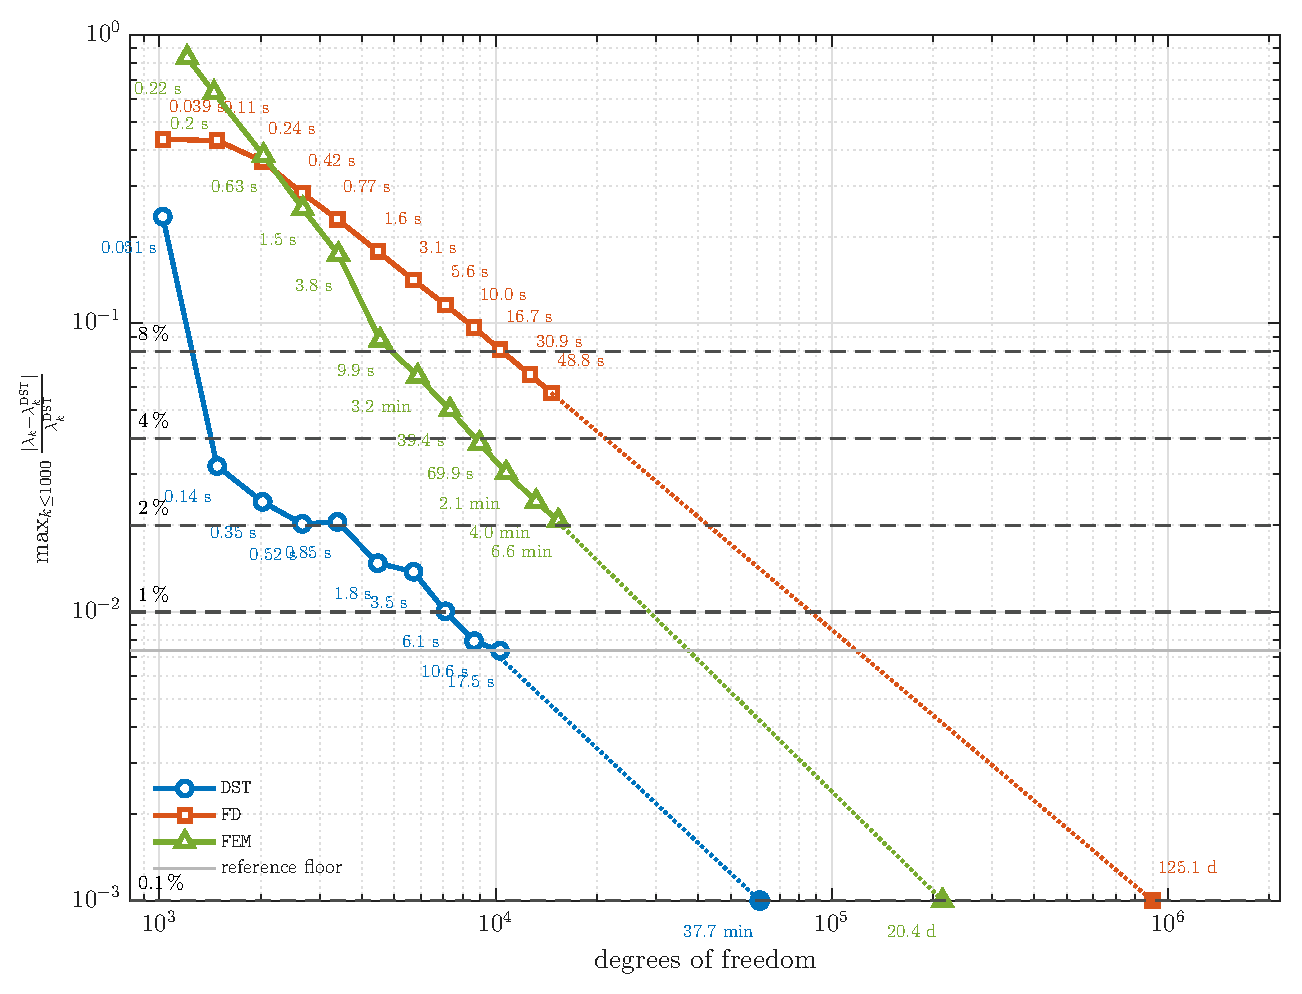
\includegraphics[width=0.85\textwidth]{ellipse_minus_quadrant_dof_requirement_n1000}
  \caption{Accuracy of the first 1000 eigenvalues of Laplace operator, zero Dirichlet boundary conditions, ellipse-minus-quadrant domain \texttt{ellipse\_minus\_quadrant}. Largest relative error over the whole block of first $1000$ eigenvalues, $\left\{ \lambda_k \right\}_{k=1}^{1000}$, $\max_{k \leq 1000} \frac{|\lambda_k - \lambda_k^{\text{DST}}|}{\lambda_k^{\text{DST}}}$, against the degrees of freedom used by each discretisation of Laplace operator, compared with the reference eigenvalues computed by \texttt{DST} with 19783 degrees of freedom. Each marker is labelled with the computation time of the particular run, dotted lines show extrapolated values.}
  \label{fig:dof_requirement_ellipse_minus_quadrant}
\end{figure}
